\documentclass[a4paper]{book}
\usepackage{a4wide}
\usepackage{makeidx}
\usepackage{graphicx}
\usepackage{multicol}
\usepackage{float}
\usepackage{listings}
\usepackage{color}
\usepackage{textcomp}
\usepackage{alltt}
\usepackage{times}
\usepackage{ifpdf}
\ifpdf
\usepackage[pdftex,
            pagebackref=true,
            colorlinks=true,
            linkcolor=blue,
            unicode
           ]{hyperref}
\else
\usepackage[ps2pdf,
            pagebackref=true,
            colorlinks=true,
            linkcolor=blue,
            unicode
           ]{hyperref}
\usepackage{pspicture}
\fi
\usepackage[utf8]{inputenc}
\usepackage{doxygen}
\lstset{language=C++,inputencoding=utf8,basicstyle=\footnotesize,breaklines=true,breakatwhitespace=true,tabsize=8,numbers=left }
\makeindex
\setcounter{tocdepth}{3}
\renewcommand{\footrulewidth}{0.4pt}
\begin{document}
\hypersetup{pageanchor=false}
\begin{titlepage}
\vspace*{7cm}
\begin{center}
{\Large Reference Manual}\\
\vspace*{1cm}
{\large Generated by Doxygen 1.6.1}\\
\vspace*{0.5cm}
{\small Fri Aug 16 15:19:38 2013}\\
\end{center}
\end{titlepage}
\clearemptydoublepage
\pagenumbering{roman}
\tableofcontents
\clearemptydoublepage
\pagenumbering{arabic}
\hypersetup{pageanchor=true}
\chapter{Class Index}
\section{Class Hierarchy}
This inheritance list is sorted roughly, but not completely, alphabetically:\begin{DoxyCompactList}
\item \contentsline{section}{fastgenematch::Genematch\_\-converter}{\pageref{classfastgenematch_1_1Genematch__converter}}{}
\begin{DoxyCompactList}
\item \contentsline{section}{fastgenematch::Genematcher}{\pageref{classfastgenematch_1_1Genematcher}}{}
\begin{DoxyCompactList}
\item \contentsline{section}{fastgenematch::Fgc\_\-proc}{\pageref{classfastgenematch_1_1Fgc__proc}}{}
\end{DoxyCompactList}
\end{DoxyCompactList}
\item \contentsline{section}{fastgenematch::Geneobject}{\pageref{classfastgenematch_1_1Geneobject}}{}
\item \contentsline{section}{fastgenematch::Hashcaller}{\pageref{classfastgenematch_1_1Hashcaller}}{}
\item \contentsline{section}{fastgenematch::Hashcaller::out128}{\pageref{unionfastgenematch_1_1Hashcaller_1_1out128}}{}
\item \contentsline{section}{fastgenematch::Genematch\_\-converter::params}{\pageref{structfastgenematch_1_1Genematch__converter_1_1params}}{}
\item \contentsline{section}{fastgenematch::Genematcher::params}{\pageref{structfastgenematch_1_1Genematcher_1_1params}}{}
\end{DoxyCompactList}

\chapter{Class Index}
\section{Class List}
Here are the classes, structs, unions and interfaces with brief descriptions:\begin{DoxyCompactList}
\item\contentsline{section}{\hyperlink{classfastgenematch_1_1Fgc__proc}{fastgenematch::Fgc\_\-proc} }{\pageref{classfastgenematch_1_1Fgc__proc}}{}
\item\contentsline{section}{\hyperlink{classfastgenematch_1_1Genematch__converter}{fastgenematch::Genematch\_\-converter} }{\pageref{classfastgenematch_1_1Genematch__converter}}{}
\item\contentsline{section}{\hyperlink{classfastgenematch_1_1Genematcher}{fastgenematch::Genematcher} }{\pageref{classfastgenematch_1_1Genematcher}}{}
\item\contentsline{section}{\hyperlink{classfastgenematch_1_1Geneobject}{fastgenematch::Geneobject} }{\pageref{classfastgenematch_1_1Geneobject}}{}
\item\contentsline{section}{\hyperlink{classfastgenematch_1_1Hashcaller}{fastgenematch::Hashcaller} }{\pageref{classfastgenematch_1_1Hashcaller}}{}
\item\contentsline{section}{\hyperlink{unionfastgenematch_1_1Hashcaller_1_1out128}{fastgenematch::Hashcaller::out128} }{\pageref{unionfastgenematch_1_1Hashcaller_1_1out128}}{}
\item\contentsline{section}{\hyperlink{structfastgenematch_1_1Genematch__converter_1_1params}{fastgenematch::Genematch\_\-converter::params} }{\pageref{structfastgenematch_1_1Genematch__converter_1_1params}}{}
\item\contentsline{section}{\hyperlink{structfastgenematch_1_1Genematcher_1_1params}{fastgenematch::Genematcher::params} }{\pageref{structfastgenematch_1_1Genematcher_1_1params}}{}
\end{DoxyCompactList}

\chapter{Class Documentation}
\hypertarget{classfastgenematch_1_1Fgc__proc}{
\section{fastgenematch::Fgc\_\-proc Class Reference}
\label{classfastgenematch_1_1Fgc__proc}\index{fastgenematch::Fgc\_\-proc@{fastgenematch::Fgc\_\-proc}}
}
Inheritance diagram for fastgenematch::Fgc\_\-proc::\begin{figure}[H]
\begin{center}
\leavevmode
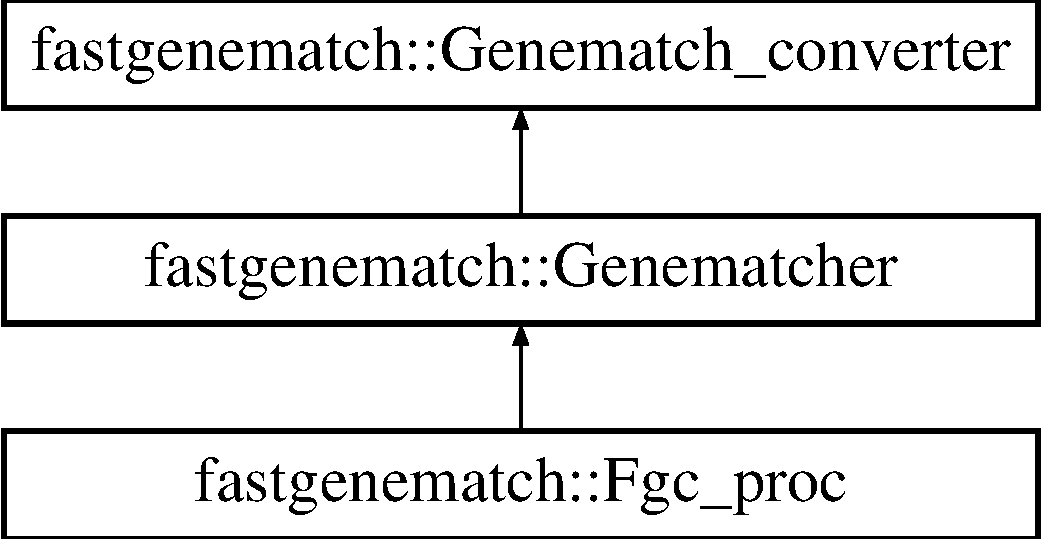
\includegraphics[height=3cm]{classfastgenematch_1_1Fgc__proc}
\end{center}
\end{figure}
\subsection*{Public Member Functions}
\begin{DoxyCompactItemize}
\item 
\hypertarget{classfastgenematch_1_1Fgc__proc_aa2e4c70c18b1bbd11ae9e8874b1f613c}{
void {\bfseries report} ()}
\label{classfastgenematch_1_1Fgc__proc_aa2e4c70c18b1bbd11ae9e8874b1f613c}

\item 
\hypertarget{classfastgenematch_1_1Fgc__proc_a7eb4de0a28fe83671cd2e1355df81ec3}{
void {\bfseries reset} ()}
\label{classfastgenematch_1_1Fgc__proc_a7eb4de0a28fe83671cd2e1355df81ec3}

\item 
\hypertarget{classfastgenematch_1_1Fgc__proc_a2bf2a1ab299c9b24e62a60ec292783b2}{
void {\bfseries bind} (const std::string \&name)}
\label{classfastgenematch_1_1Fgc__proc_a2bf2a1ab299c9b24e62a60ec292783b2}

\item 
\hypertarget{classfastgenematch_1_1Fgc__proc_a76fe9f3ccc083ed767e687d131c301b6}{
void {\bfseries main} ()}
\label{classfastgenematch_1_1Fgc__proc_a76fe9f3ccc083ed767e687d131c301b6}

\end{DoxyCompactItemize}


The documentation for this class was generated from the following file:\begin{DoxyCompactItemize}
\item 
fastgenematch\_\-proc.h\end{DoxyCompactItemize}

\hypertarget{classfastgenematch_1_1Genematch__converter}{
\section{fastgenematch::Genematch\_\-converter Class Reference}
\label{classfastgenematch_1_1Genematch__converter}\index{fastgenematch::Genematch\_\-converter@{fastgenematch::Genematch\_\-converter}}
}
Inheritance diagram for fastgenematch::Genematch\_\-converter::\begin{figure}[H]
\begin{center}
\leavevmode
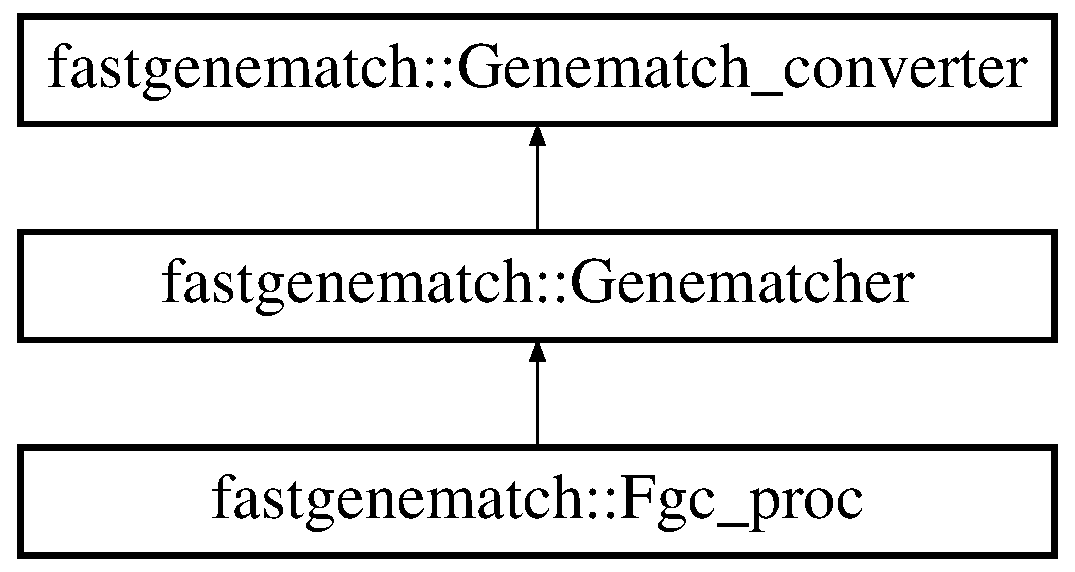
\includegraphics[height=3cm]{classfastgenematch_1_1Genematch__converter}
\end{center}
\end{figure}
\subsection*{Classes}
\begin{DoxyCompactItemize}
\item 
struct \hyperlink{structfastgenematch_1_1Genematch__converter_1_1params}{params}
\end{DoxyCompactItemize}
\subsection*{Public Member Functions}
\begin{DoxyCompactItemize}
\item 
\hypertarget{classfastgenematch_1_1Genematch__converter_a938d1c275e3a693759615fadc1738dcd}{
void {\bfseries initialize} ()}
\label{classfastgenematch_1_1Genematch__converter_a938d1c275e3a693759615fadc1738dcd}

\item 
\hypertarget{classfastgenematch_1_1Genematch__converter_a9be3e65398d049c75025a36a55e12ca4}{
void {\bfseries do\_\-convert} ()}
\label{classfastgenematch_1_1Genematch__converter_a9be3e65398d049c75025a36a55e12ca4}

\item 
\hypertarget{classfastgenematch_1_1Genematch__converter_a9e95e1ac101beafbe65c01ee7d1e5134}{
std::istream \& {\bfseries operator$<$$<$} (std::istream \&)}
\label{classfastgenematch_1_1Genematch__converter_a9e95e1ac101beafbe65c01ee7d1e5134}

\item 
\hypertarget{classfastgenematch_1_1Genematch__converter_af38195c890cb992760b8164a2ad596d8}{
std::ostream \& {\bfseries operator$>$$>$} (std::ostream \&)}
\label{classfastgenematch_1_1Genematch__converter_af38195c890cb992760b8164a2ad596d8}

\end{DoxyCompactItemize}
\subsection*{Public Attributes}
\begin{DoxyCompactItemize}
\item 
\hypertarget{classfastgenematch_1_1Genematch__converter_a8005b5b0aeae31f2d360e6b055c94021}{
\hyperlink{structfastgenematch_1_1Genematch__converter_1_1params}{params} {\bfseries param}}
\label{classfastgenematch_1_1Genematch__converter_a8005b5b0aeae31f2d360e6b055c94021}

\item 
\hypertarget{classfastgenematch_1_1Genematch__converter_a5fc827f8b0b9cdfa0568a3659eaecc8f}{
\hyperlink{classfastgenematch_1_1Geneobject}{Geneobject} {\bfseries table}}
\label{classfastgenematch_1_1Genematch__converter_a5fc827f8b0b9cdfa0568a3659eaecc8f}

\item 
\hypertarget{classfastgenematch_1_1Genematch__converter_a1dda29ed6052d0134e2b3d4a66299b44}{
std::string {\bfseries title}}
\label{classfastgenematch_1_1Genematch__converter_a1dda29ed6052d0134e2b3d4a66299b44}

\item 
\hypertarget{classfastgenematch_1_1Genematch__converter_aae4e4312aa893f5278b67115100b6364}{
std::unordered\_\-map$<$ std::string, format\_\-types $>$ {\bfseries lookup}}
\label{classfastgenematch_1_1Genematch__converter_aae4e4312aa893f5278b67115100b6364}

\end{DoxyCompactItemize}


The documentation for this class was generated from the following files:\begin{DoxyCompactItemize}
\item 
fastgenematch.h\item 
fastgenematch.cpp\end{DoxyCompactItemize}

\hypertarget{classfastgenematch_1_1Genematcher}{
\section{fastgenematch::Genematcher Class Reference}
\label{classfastgenematch_1_1Genematcher}\index{fastgenematch::Genematcher@{fastgenematch::Genematcher}}
}
Inheritance diagram for fastgenematch::Genematcher::\begin{figure}[H]
\begin{center}
\leavevmode
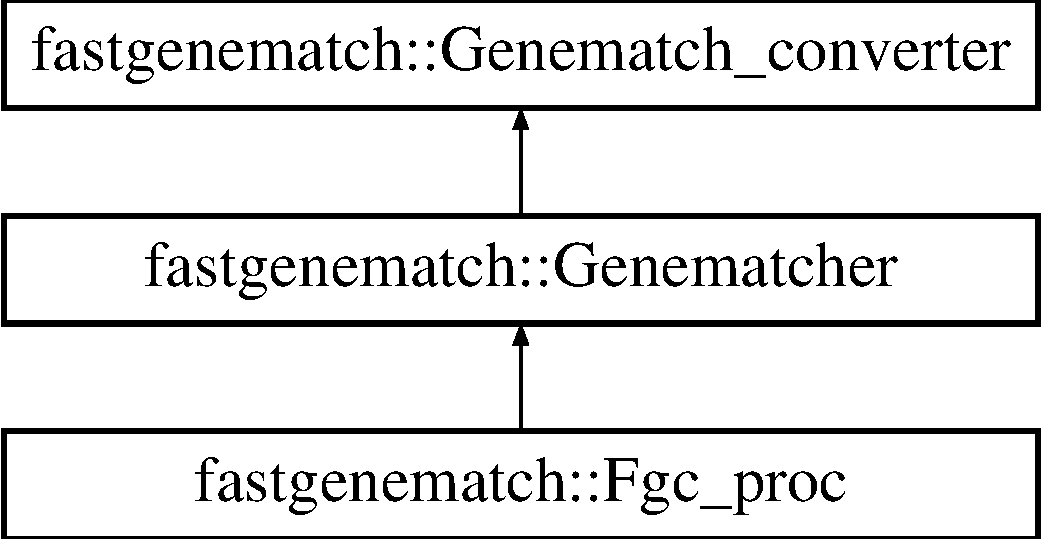
\includegraphics[height=3cm]{classfastgenematch_1_1Genematcher}
\end{center}
\end{figure}
\subsection*{Classes}
\begin{DoxyCompactItemize}
\item 
struct \hyperlink{structfastgenematch_1_1Genematcher_1_1params}{params}
\end{DoxyCompactItemize}
\subsection*{Public Member Functions}
\begin{DoxyCompactItemize}
\item 
\hypertarget{classfastgenematch_1_1Genematcher_a84c8e20ee330e41d997e2f898fd5e05b}{
void {\bfseries print\_\-help} ()}
\label{classfastgenematch_1_1Genematcher_a84c8e20ee330e41d997e2f898fd5e05b}

\item 
\hypertarget{classfastgenematch_1_1Genematcher_a8ca976f27e2e3a12d3e8355b38db096a}{
void {\bfseries print\_\-settings} ()}
\label{classfastgenematch_1_1Genematcher_a8ca976f27e2e3a12d3e8355b38db096a}

\item 
\hypertarget{classfastgenematch_1_1Genematcher_aa8e3bdaa3e1ae1bb7b90ebf5a9a6b50a}{
void {\bfseries print\_\-version} ()}
\label{classfastgenematch_1_1Genematcher_aa8e3bdaa3e1ae1bb7b90ebf5a9a6b50a}

\item 
\hypertarget{classfastgenematch_1_1Genematcher_ad22d1197cc39ff29fc5a805b5c505ac8}{
void {\bfseries validate} ()}
\label{classfastgenematch_1_1Genematcher_ad22d1197cc39ff29fc5a805b5c505ac8}

\item 
\hypertarget{classfastgenematch_1_1Genematcher_af180d9099b7f0b5a30931ebfd8fbf175}{
void {\bfseries match} ()}
\label{classfastgenematch_1_1Genematcher_af180d9099b7f0b5a30931ebfd8fbf175}

\item 
\hypertarget{classfastgenematch_1_1Genematcher_a197cab88ac897087571155214f81a91e}{
void {\bfseries match\_\-pair} ()}
\label{classfastgenematch_1_1Genematcher_a197cab88ac897087571155214f81a91e}

\item 
\hypertarget{classfastgenematch_1_1Genematcher_a2465b9937753e710d5373dbad2d4e2e1}{
bool {\bfseries read} (int argc, char $\ast$$\ast$argv)}
\label{classfastgenematch_1_1Genematcher_a2465b9937753e710d5373dbad2d4e2e1}

\item 
\hypertarget{classfastgenematch_1_1Genematcher_af6c777f817710746ed7f41509e6086d4}{
const std::string {\bfseries feedin} ()}
\label{classfastgenematch_1_1Genematcher_af6c777f817710746ed7f41509e6086d4}

\item 
\hypertarget{classfastgenematch_1_1Genematcher_a2608215c7b1c6f6f43c19e6117963bf9}{
void {\bfseries feedout} (const std::ostringstream \&)}
\label{classfastgenematch_1_1Genematcher_a2608215c7b1c6f6f43c19e6117963bf9}

\item 
\hypertarget{classfastgenematch_1_1Genematcher_a846f651c279bf62c7fe305884a37c7cd}{
bool {\bfseries main} (int argc, char $\ast$$\ast$argv)}
\label{classfastgenematch_1_1Genematcher_a846f651c279bf62c7fe305884a37c7cd}

\end{DoxyCompactItemize}
\subsection*{Public Attributes}
\begin{DoxyCompactItemize}
\item 
\hypertarget{classfastgenematch_1_1Genematcher_ad79b2b34f9b424f29e4ecc6bfe7bfefb}{
\hyperlink{structfastgenematch_1_1Genematch__converter_1_1params}{params} {\bfseries settings}}
\label{classfastgenematch_1_1Genematcher_ad79b2b34f9b424f29e4ecc6bfe7bfefb}

\end{DoxyCompactItemize}


The documentation for this class was generated from the following files:\begin{DoxyCompactItemize}
\item 
fastgenematch.h\item 
fastgenematch.cpp\end{DoxyCompactItemize}

\hypertarget{classfastgenematch_1_1Geneobject}{
\section{fastgenematch::Geneobject Class Reference}
\label{classfastgenematch_1_1Geneobject}\index{fastgenematch::Geneobject@{fastgenematch::Geneobject}}
}
\subsection*{Public Types}
\begin{DoxyCompactItemize}
\item 
\hypertarget{classfastgenematch_1_1Geneobject_ad1dce72c4d21326253829528c921c97b}{
typedef std::shared\_\-ptr$<$ std::unordered\_\-map$<$ std::string, std::string, \hyperlink{classfastgenematch_1_1Hashcaller}{Hashcaller} $>$ $>$ {\bfseries hashtable}}
\label{classfastgenematch_1_1Geneobject_ad1dce72c4d21326253829528c921c97b}

\item 
\hypertarget{classfastgenematch_1_1Geneobject_ab900fe6b1116e8d5b4f2f62e7d45d1f7}{
typedef std::unordered\_\-map$<$ std::string, std::string, \hyperlink{classfastgenematch_1_1Hashcaller}{Hashcaller} $>$ {\bfseries \_\-hashtable}}
\label{classfastgenematch_1_1Geneobject_ab900fe6b1116e8d5b4f2f62e7d45d1f7}

\end{DoxyCompactItemize}
\subsection*{Public Member Functions}
\begin{DoxyCompactItemize}
\item 
\hypertarget{classfastgenematch_1_1Geneobject_a69326e96a8d2cdfedee2c44f3ca2eb0b}{
std::string \& {\bfseries operator\mbox{[}$\,$\mbox{]}} (const std::string \&key)}
\label{classfastgenematch_1_1Geneobject_a69326e96a8d2cdfedee2c44f3ca2eb0b}

\item 
\hypertarget{classfastgenematch_1_1Geneobject_a5d0fad4b7c244be239901c6e794cf1f5}{
std::string \& {\bfseries operator()} (const std::string \&key)}
\label{classfastgenematch_1_1Geneobject_a5d0fad4b7c244be239901c6e794cf1f5}

\item 
\hypertarget{classfastgenematch_1_1Geneobject_a2542e61f0e78690217e94e89c386ec24}{
uint32\_\-t {\bfseries getseed} ()}
\label{classfastgenematch_1_1Geneobject_a2542e61f0e78690217e94e89c386ec24}

\item 
\hypertarget{classfastgenematch_1_1Geneobject_a775dded873cb868027048baee7fce0a9}{
void {\bfseries rehash} ()}
\label{classfastgenematch_1_1Geneobject_a775dded873cb868027048baee7fce0a9}

\item 
\hypertarget{classfastgenematch_1_1Geneobject_a36e67a37874e46d4655d8e688d975852}{
void {\bfseries reseed} ()}
\label{classfastgenematch_1_1Geneobject_a36e67a37874e46d4655d8e688d975852}

\item 
\hypertarget{classfastgenematch_1_1Geneobject_ad1359c68213e594b5aa600bff1e10f64}{
void {\bfseries setseed} (const uint32\_\-t \&in)}
\label{classfastgenematch_1_1Geneobject_ad1359c68213e594b5aa600bff1e10f64}

\item 
\hypertarget{classfastgenematch_1_1Geneobject_a4dd2f125e2915ee2c59b09f20e329721}{
void {\bfseries serialize} ()}
\label{classfastgenematch_1_1Geneobject_a4dd2f125e2915ee2c59b09f20e329721}

\item 
\hypertarget{classfastgenematch_1_1Geneobject_a23178da06dc9ff52d58a7d3ba7e87a76}{
void {\bfseries serialize} (const std::string \&)}
\label{classfastgenematch_1_1Geneobject_a23178da06dc9ff52d58a7d3ba7e87a76}

\item 
\hypertarget{classfastgenematch_1_1Geneobject_a4532439959e22fb1618dd240a382d313}{
void {\bfseries load} (const std::string \&)}
\label{classfastgenematch_1_1Geneobject_a4532439959e22fb1618dd240a382d313}

\item 
\hypertarget{classfastgenematch_1_1Geneobject_a4bab27f711113a8f86066c1b40491d18}{
void {\bfseries load} ()}
\label{classfastgenematch_1_1Geneobject_a4bab27f711113a8f86066c1b40491d18}

\end{DoxyCompactItemize}
\subsection*{Public Attributes}
\begin{DoxyCompactItemize}
\item 
\hypertarget{classfastgenematch_1_1Geneobject_ac1da8f2a744493726da5a2fbaef4f709}{
std::pair$<$ int, int $>$ {\bfseries formats}}
\label{classfastgenematch_1_1Geneobject_ac1da8f2a744493726da5a2fbaef4f709}

\item 
\hypertarget{classfastgenematch_1_1Geneobject_a3e6684c3c20db786ccec541e136afa8c}{
hashtable {\bfseries data}}
\label{classfastgenematch_1_1Geneobject_a3e6684c3c20db786ccec541e136afa8c}

\end{DoxyCompactItemize}
\subsection*{Protected Attributes}
\begin{DoxyCompactItemize}
\item 
\hypertarget{classfastgenematch_1_1Geneobject_a45670e89f2e7c70136b8d69027e9972c}{
size\_\-t {\bfseries length}}
\label{classfastgenematch_1_1Geneobject_a45670e89f2e7c70136b8d69027e9972c}

\item 
\hypertarget{classfastgenematch_1_1Geneobject_a60d4a4d6321022fd74d57b390e645e75}{
std::string {\bfseries empty}}
\label{classfastgenematch_1_1Geneobject_a60d4a4d6321022fd74d57b390e645e75}

\item 
\hypertarget{classfastgenematch_1_1Geneobject_afdb66b5183b05f3c15f6b73f691e8b57}{
uint32\_\-t {\bfseries seed}}
\label{classfastgenematch_1_1Geneobject_afdb66b5183b05f3c15f6b73f691e8b57}

\end{DoxyCompactItemize}


The documentation for this class was generated from the following files:\begin{DoxyCompactItemize}
\item 
fastgenematch.h\item 
fastgenematch.cpp\end{DoxyCompactItemize}

\hypertarget{classfastgenematch_1_1Hashcaller}{
\section{fastgenematch::Hashcaller Class Reference}
\label{classfastgenematch_1_1Hashcaller}\index{fastgenematch::Hashcaller@{fastgenematch::Hashcaller}}
}
\subsection*{Classes}
\begin{DoxyCompactItemize}
\item 
union \hyperlink{unionfastgenematch_1_1Hashcaller_1_1out128}{out128}
\end{DoxyCompactItemize}
\subsection*{Public Member Functions}
\begin{DoxyCompactItemize}
\item 
\hypertarget{classfastgenematch_1_1Hashcaller_adb7b8084b445f24f0fc412cb7de3566e}{
size\_\-t {\bfseries operator()} (const std::string \&key) const }
\label{classfastgenematch_1_1Hashcaller_adb7b8084b445f24f0fc412cb7de3566e}

\end{DoxyCompactItemize}
\subsection*{Static Public Attributes}
\begin{DoxyCompactItemize}
\item 
\hypertarget{classfastgenematch_1_1Hashcaller_af087bfe64d5b7cb0251a19071b26a21e}{
static uint32\_\-t {\bfseries seed} = SEED}
\label{classfastgenematch_1_1Hashcaller_af087bfe64d5b7cb0251a19071b26a21e}

\end{DoxyCompactItemize}
\subsection*{Protected Attributes}
\begin{DoxyCompactItemize}
\item 
\hypertarget{classfastgenematch_1_1Hashcaller_a243ace8edfd79fd39900fb34aafa593e}{
union \hyperlink{unionfastgenematch_1_1Hashcaller_1_1out128}{out128} {\bfseries out}}
\label{classfastgenematch_1_1Hashcaller_a243ace8edfd79fd39900fb34aafa593e}

\end{DoxyCompactItemize}


The documentation for this class was generated from the following files:\begin{DoxyCompactItemize}
\item 
fastgenematch.h\item 
fastgenematch.cpp\end{DoxyCompactItemize}

\hypertarget{unionfastgenematch_1_1Hashcaller_1_1out128}{
\section{fastgenematch::Hashcaller::out128 Union Reference}
\label{unionfastgenematch_1_1Hashcaller_1_1out128}\index{fastgenematch::Hashcaller::out128@{fastgenematch::Hashcaller::out128}}
}
\subsection*{Public Attributes}
\begin{DoxyCompactItemize}
\item 
\hypertarget{unionfastgenematch_1_1Hashcaller_1_1out128_ab3cfe6bc66359064c054b3cb499f349c}{
size\_\-t {\bfseries s}}
\label{unionfastgenematch_1_1Hashcaller_1_1out128_ab3cfe6bc66359064c054b3cb499f349c}

\item 
\hypertarget{unionfastgenematch_1_1Hashcaller_1_1out128_a3787f3897a3825707dfae44257e44d16}{
uint64\_\-t {\bfseries t} \mbox{[}2\mbox{]}}
\label{unionfastgenematch_1_1Hashcaller_1_1out128_a3787f3897a3825707dfae44257e44d16}

\end{DoxyCompactItemize}


The documentation for this union was generated from the following file:\begin{DoxyCompactItemize}
\item 
fastgenematch.h\end{DoxyCompactItemize}

\hypertarget{structfastgenematch_1_1Genematch__converter_1_1params}{
\section{fastgenematch::Genematch\_\-converter::params Struct Reference}
\label{structfastgenematch_1_1Genematch__converter_1_1params}\index{fastgenematch::Genematch\_\-converter::params@{fastgenematch::Genematch\_\-converter::params}}
}
\subsection*{Public Attributes}
\begin{DoxyCompactItemize}
\item 
\hypertarget{structfastgenematch_1_1Genematch__converter_1_1params_a7e1e7c2de3616fcb90c7581b6063c7e7}{
std::string {\bfseries outputname}}
\label{structfastgenematch_1_1Genematch__converter_1_1params_a7e1e7c2de3616fcb90c7581b6063c7e7}

\item 
\hypertarget{structfastgenematch_1_1Genematch__converter_1_1params_a86f639bede2c1b30e26d01fa3af49abc}{
std::string {\bfseries inputformat}}
\label{structfastgenematch_1_1Genematch__converter_1_1params_a86f639bede2c1b30e26d01fa3af49abc}

\item 
\hypertarget{structfastgenematch_1_1Genematch__converter_1_1params_afbfff345aab934eda4c4760cfb6ab453}{
std::string {\bfseries outputformat}}
\label{structfastgenematch_1_1Genematch__converter_1_1params_afbfff345aab934eda4c4760cfb6ab453}

\end{DoxyCompactItemize}


The documentation for this struct was generated from the following file:\begin{DoxyCompactItemize}
\item 
fastgenematch.h\end{DoxyCompactItemize}

\hypertarget{structfastgenematch_1_1Genematcher_1_1params}{
\section{fastgenematch::Genematcher::params Struct Reference}
\label{structfastgenematch_1_1Genematcher_1_1params}\index{fastgenematch::Genematcher::params@{fastgenematch::Genematcher::params}}
}
\subsection*{Public Attributes}
\begin{DoxyCompactItemize}
\item 
\hypertarget{structfastgenematch_1_1Genematcher_1_1params_afe18ab3df28ac792ceafd23c762e60e9}{
bool {\bfseries hold}}
\label{structfastgenematch_1_1Genematcher_1_1params_afe18ab3df28ac792ceafd23c762e60e9}

\item 
\hypertarget{structfastgenematch_1_1Genematcher_1_1params_af71f71258871265c22ee2926c62c8e44}{
bool {\bfseries bin}}
\label{structfastgenematch_1_1Genematcher_1_1params_af71f71258871265c22ee2926c62c8e44}

\item 
\hypertarget{structfastgenematch_1_1Genematcher_1_1params_a592916e8189b43e5e48eb6ecbf8a5c4f}{
bool {\bfseries pair}}
\label{structfastgenematch_1_1Genematcher_1_1params_a592916e8189b43e5e48eb6ecbf8a5c4f}

\item 
\hypertarget{structfastgenematch_1_1Genematcher_1_1params_a4ca5d6d173f9f68ef45c6a5da14ce02c}{
bool {\bfseries verbose}}
\label{structfastgenematch_1_1Genematcher_1_1params_a4ca5d6d173f9f68ef45c6a5da14ce02c}

\item 
\hypertarget{structfastgenematch_1_1Genematcher_1_1params_a70798746749ae929cda854f45eb7d495}{
bool {\bfseries validate}}
\label{structfastgenematch_1_1Genematcher_1_1params_a70798746749ae929cda854f45eb7d495}

\item 
\hypertarget{structfastgenematch_1_1Genematcher_1_1params_a6d9a31d418eb6714c47e4593dcab2063}{
bool {\bfseries filein}}
\label{structfastgenematch_1_1Genematcher_1_1params_a6d9a31d418eb6714c47e4593dcab2063}

\item 
\hypertarget{structfastgenematch_1_1Genematcher_1_1params_ad87dee81e835b9541de62f7db968cd1c}{
bool {\bfseries give\_\-keys}}
\label{structfastgenematch_1_1Genematcher_1_1params_ad87dee81e835b9541de62f7db968cd1c}

\item 
\hypertarget{structfastgenematch_1_1Genematcher_1_1params_ab3fce4dd57241d4c0f27fd13866c3a6e}{
bool {\bfseries give\_\-vals}}
\label{structfastgenematch_1_1Genematcher_1_1params_ab3fce4dd57241d4c0f27fd13866c3a6e}

\item 
\hypertarget{structfastgenematch_1_1Genematcher_1_1params_a9aa5e818a4b9b22667c675c652046ba2}{
bool {\bfseries give\_\-pairs}}
\label{structfastgenematch_1_1Genematcher_1_1params_a9aa5e818a4b9b22667c675c652046ba2}

\item 
\hypertarget{structfastgenematch_1_1Genematcher_1_1params_a13581b681e428bd1109e1d952faa803a}{
std::string {\bfseries fname}}
\label{structfastgenematch_1_1Genematcher_1_1params_a13581b681e428bd1109e1d952faa803a}

\item 
\hypertarget{structfastgenematch_1_1Genematcher_1_1params_a03105d36fbe64f6dc2b38c82e57e76f4}{
std::string {\bfseries binname}}
\label{structfastgenematch_1_1Genematcher_1_1params_a03105d36fbe64f6dc2b38c82e57e76f4}

\item 
\hypertarget{structfastgenematch_1_1Genematcher_1_1params_afa74b1a4c19be53b61aac3e6fff59855}{
bool {\bfseries convert}}
\label{structfastgenematch_1_1Genematcher_1_1params_afa74b1a4c19be53b61aac3e6fff59855}

\item 
\hypertarget{structfastgenematch_1_1Genematcher_1_1params_adbf4e2c1fc035d3f5d62519d91a814ca}{
bool {\bfseries fileout}}
\label{structfastgenematch_1_1Genematcher_1_1params_adbf4e2c1fc035d3f5d62519d91a814ca}

\end{DoxyCompactItemize}


The documentation for this struct was generated from the following file:\begin{DoxyCompactItemize}
\item 
fastgenematch.h\end{DoxyCompactItemize}

\printindex
\end{document}
